\chapter{Event Reconstruction}
\label{ch:RecoCal}

The most basic form of raw data collected is a vector of hits above threshold. The MC simulation described in chapter \ref{ch:Simulation} also outputs events in this format. However, these objects by themselves are not very useful; instead, a certain level of reconstruction is required before real physics can be studied. The first major step in this process is to apply calibration so that the hits can be translated into a set of energy depositions, consistent throughout and across both detectors. Any number of algorithms can then be applied to create new objects or search for features, including tracks, the event vertex, or particle identifiers (PIDs). This chapter describes the calibration and elements of the reconstruction chain relevant to the NC disappearance analysis.

\section{Calibration}
\label{sec:Calib}

The purpose of calibration is to ensure a uniform detector response throughout each and across both detectors. This is done in two major steps, a relative and absolute calibration. The relative calibration accounts for threshold effects and attenuation across a single cell. It is designed to create a uniform response throughout a cell and across a single detector. The absolute calibration creates a scale factor for each detector to convert the calibrated PE scale from the relative calibration into an energy unit. This section follows the SA notes in reference \cite{ref:TNCalib}.

\subsection{Relative Calibration}
\label{sec:CalibRel}

The relative calibration is designed to convert the PE signal output from the electronics into a calibrated unit, such that two equal signals from any two detector locations mean equal true energy deposited. This part of the calibration accounts for threshold effects and attenuation in the WLS fibers, outputting a corrected PE value, the PECorr.

Hits from through-going cosmic ray muons, or muons that enter and exit the detector without stopping, are used for the relative calibration. The WindowTrack algorithm, a fast algorithm that fits straight lines through hits \cite{ref:RecoWinTrack}, is used to produce $3$D tracks from the cosmic ray events, and only those with a successful reconstruction are used. Within these events, only tricell hits are used for the calibration procedure. A tricell hit is defined as a hit in cell $i$ within a given plane that also has hits in cells $i+1$ and $i-1$. Under special circumstances (low statistics, too many dead neighboring cells) different hits are used for a particular cell. The path length of the cosmic traveling through the cell and the distance from readout are calculated for all of the selected hits in a cell. The distance from readout is labeled $W$, an alias for either X or Y, such that $W = 0$ is the center of a cell and positive values of $W$ are closer to the readout. From this information, individual histograms of the average PE/cm vs $W$ are constructed for each cell. The relative calibration procedures apply corrections to these histograms.

The first effect handled by the relative calibration is of threshold and shielding. Thresholds refer to the issue that an energy deposition may not register for a hit at all, as opposed to simply being attenuated, if there are not enough photons that reach the APD. Shielding refers to the tendency of the detector mass to alter the average signal of a minimum ionizing particle, or MIP, as a function of distance to the readout. Both of these effects would bias the set of hits used by the calibration by preferably selecting hits with greater numbers of photons, in turn underestimating the true energy deposited in the cell. To account for this, a correction factor is applied for each cell,
\beq
T = \frac{PE}{\lambda} \cdot \frac{E_{True}}{E_{MIP}}
\label{eq:CalibThreshold}
\eeq

\n where $T$ is correction factor, $PE$ is the number of simulated photons that the electronics register, $\lambda$ is the number of photons that would be seen without fluctuations, $E_{True}$ is the true energy deposited in the scintillator, and $E_{MIP}$ is the energy that would be deposited based only on the particle path length through the cell. The ratio on the left accounts for the threshold correction since $\lambda$ is only dependent on the simulated threshold level, and the ratio on the right accounts for the shielding correction since $E_{MIP}$ is only depenedent on the path length. Two dimensional histograms of the correction factor as a function of the cell number and distance from the readout are made for each detector and view, then fit with a polynomial to remove noise. These histograms are then used to correct the corresponding data and MC. Figure \ref{fig:CalibThreshold} shows examples of this correction factor used for the FD.
\begin{figure}[htb]
  \centering
  \begin{tabular}{c c}
    \includegraphics[width=.47\textwidth]{figures/Calib/ThresholdFDX.png} &
    \includegraphics[width=.47\textwidth]{figures/Calib/ThresholdFDY.png} \\
  \end{tabular}
  \caption[Threshold and Shielding Correction Factors]{Correction factor for threshold and shielding effects at the FD as a function of cell number and distance from electronic readout. Cells in the X view are shown on the left, Y view on the right.}
  \label{fig:CalibThreshold}
\end{figure}

The next part of the relative calibration is the general form of the attenuation correction. Tricell hits are grouped by cell and fit to a double exponential to consider both short and long path light. For data, individual fits are performed for every single cell. In MC, a fit is performed on the group of all cells in a particular view and at the same location in a plane due to much lower simulated cosmic event statistics. The double exponential has the form
\beq
y = C + A\left(\exp\left(\frac{W}{X}\right) + \exp\left(-\frac{L+W}{X}\right)\right)
\label{eq:CalibAttenuation}
\eeq

\n where $C$, $A$, and $X$ are the free parameters, and $L$ is the full length of the cell. $X$ is the cell attenuation length. The fit excludes hits in the regions closest and furthest to the readout. It includes the range $[-750, 750]$ at the FD, $[-150, 150]$ for the fully active region of the ND and for Y view muon catcher cells, and $[-150, 50]$ for X view muon catcher cells, with all numbers in cm. These central regions are chosen to exclude the significant rolloff regions at the end of the cells, which are handled differently.

The final step in the relative calibration handles the attenuation correction at the ends of the cells and the residuals from the fit above in the central part of the cells. First, both of these regions are fit with a single LOWESS curve using a tricube weight,
\beq
w_i = \begin{cases}
\left(1 - \left| \frac{W - W_i}{\sigma} \right|^3 \right)^3 & \mbox{for } \vert W - W_i \vert < \sigma \\
0 & \mbox{for } \vert W - W_i \vert \geq \sigma \end{cases}
\label{eq:CalibRolloff}
\eeq

\n where $W$ is a local point on the curve, $W_i$ is the $i$th neighbor of the local point, $w_i$ is the weight on $W_i$, and $\sigma = 30\unit{cm}$ is the range of neighbors that affect the value of $W$. $W$ is then the weighted mean of $W_i$. Next, a simple line of the form $y = mW + c$ is fit to a collection of the neighbor points around a point, $W$, to give the corrected response, $y$. The full LOWESS curve is approximated by linear interpolation between $20$ points calculated using this procedure. The full attenuation calibration combines the results of the linear interpolation with the result of the double exponential above. Figure \ref{fig:CalibAttenuation} shows examples of the fully fit attenuation curves used in FD data calibration.
\begin{figure}[p]
  \centering
  \begin{tabular}{c c}
    \includegraphics[width=.47\textwidth]{figures/Calib/AttenuationFDH.png} &
    \includegraphics[width=.47\textwidth]{figures/Calib/AttenuationFDV.png} \\
  \end{tabular}
  \caption[Attenuation Fits]{Fits to the average detector response for a cell in the FD. The red curves show just the result from the double exponential fit, and the blue curves show the full fit that also includes the LOWESS correction. The left plot is an example of a horizontal view cell, the right plot is an example of a vertical view cell.}
  \label{fig:CalibAttenuation}
\end{figure}

The relative calibration combines the results of all three steps to create a uniform detector response as a function of distance to readout. Figure \ref{fig:CalibRelative} shows the MC before and after calibration is applied to assess the performance of the full procedure. The regions with deviations at the end of the cells ultimately are not used for the analysis.
\begin{figure}[p]
  \centering
  \begin{tabular}{c c}
    \includegraphics[width=.47\textwidth]{figures/Calib/RelativeNDX.png} &
    \includegraphics[width=.47\textwidth]{figures/Calib/RelativeNDY.png} \\
    \includegraphics[width=.47\textwidth]{figures/Calib/RelativeFDX.png} &
    \includegraphics[width=.47\textwidth]{figures/Calib/RelativeFDY.png} \\
  \end{tabular}
  \caption[Relative Calibration Results]{Ratios of mean reconstructed to true energy as a function of distance to readout to assess the performance of the relative calibration. The red points show the ratios before calibration; the blue points after. The left column shows calibration of the X view cells, the right column shows the Y view cells, the top row shows the ND relative calibration results, and the bottom shows the FD results.}
  \label{fig:CalibRelative}
\end{figure}

\subsection{Absolute Calibration}
\label{sec:CalibAbs}

The absolute calibration is performed after the relative calibration to convert the corrected PE signal into an energy value. Much like the relative calibration, the absolute calibration uses a sample of tricell hits from cosmic ray muons. However, in this case the energy deposited in the cell must be known in order to convert the PE signal into an energy. The energy is known either from external sources \cite{ref:MuonTables} or the Bethe-Block equation \cite{ref:PDG},
\beq
\left\langle-\frac{dE}{dx} \right\rangle = Kz^2 \frac{Z}{A} \frac{1}{\beta^2} \left[ \frac{1}{2} \ln \frac{2 m_e c^2 \beta^2 \gamma^2 W_{max}}{I^2} - \beta^2 - \frac{\delta(\beta\gamma)}{2} \right],
\label{eq:BetheBlock}
\eeq

\n where $K \equiv 4\pi N_A r^2_e m_e c^2$, $r_e$ is the classical electron radius, $m_e c^2$ is the electron rest energy, $z$ is the charge number of the incident particle, $Z$ and $A$ are the atomic number and mass of the stopping material, $\beta$ and $\gamma$ are calculated for the incident particle, $W_{max}$ is the maximum energy transfer to an electron in a single collision, $I$ is the mean excitation energy of electrons in the stopping material, and $\delta(\beta\gamma)$ is the density effect correction to ionization energy loss in the stopping material. With known energy deposition and number of PEs, determining the calibration energy scale is a simple procedure.

The particular energy used for the absolute calibration is the minimum energy deposition of muons through liquid scintillator. For \nova, the liquid scintillator is well approximated as chains of polyethylene, or (C$_{2}$H$_{4}$)\textsubscript{n}, for which muons have a minimum average energy loss of $2.079\unit{MeV}$ cm\textsuperscript{2}/g \cite{ref:MuonTables}. The density of the scintillator was measured to be $0.8617\unit{g/cm\textsuperscript{3}}$ \cite{ref:DensityScint}, giving an average energy loss per unit length of $1.792\unit{MeV/cm}$. From simulation, it was determined that this minimum energy deposition occurs between $100 - 200\unit{cm}$ from the end of a muon track, with only a $1.8\%$ variation throughout that region. Figure \ref{fig:CalibAbsDists} shows the distributions of the relative calibration corrected response as a function of distance from the muon track end for FD data and MC and the true energy deposition for the MC.
\begin{figure}[htb]
  \centering
  \begin{tabular}{c c}
    \includegraphics[width=.47\textwidth]{figures/Calib/AbsFDMCPECorrcm.png} &
    \includegraphics[width=.47\textwidth]{figures/Calib/AbsFDDataPECorrcm.png} \\
    \includegraphics[width=.47\textwidth]{figures/Calib/AbsFDMCdEdx.png} & \\
  \end{tabular}
  \caption[Detector Response to Stopping Cosmic Muons vs Distance to Track End]{Distribution of tricell hits from cosmic ray muon tracks at the FD as a function of distance to the end of the muon track. The top row shows the response in PECorr for both data and MC. The bottom left plot shows the true energy deposited for the MC.}
  \label{fig:CalibAbsDists}
\end{figure}

The absolute calibration energy scale is determined from distributions of tricell hits from stopping muons that occur between $100$ and $200\unit{cm}$ from the end of the muon track. These hits are used to make one dimensional muon energy unit (MEU) distributions of the relative calibration corrected detector response for data and MC called MEU\textsubscript{reco}, and the true energy deposition for MC called MEU\textsubscript{truth}. The calorimetric energy scale is then taken as the mean of the MEU\textsubscript{truth} distribution over the mean of the MEU\textsubscript{reco} distribution. Figure \ref{fig:CalibAbs} shows the distributions of the corrected detector response before the absolute calibration is applied, and the energy distributions after the absolute calibration is applied.
\begin{figure}[htb]
  \centering
  \begin{tabular}{c c}
    \includegraphics[width=.47\textwidth]{figures/Calib/DataMCNDPECorr.png} &
    \includegraphics[width=.47\textwidth]{figures/Calib/DataMCNDdEdx.png} \\
    \includegraphics[width=.47\textwidth]{figures/Calib/DataMCFDPECorr.png} &
    \includegraphics[width=.47\textwidth]{figures/Calib/DataMCFDdEdx.png} \\
  \end{tabular}
  \caption[Absolute Calibration Results]{Distributions of the tricell hits from cosmic ray muons $100-200\unit{cm}$ from the end of the track. The left column shows the relative calibration corrected detector response before the absolute calibration is applied. The right column shows the absolute calibrated energy deposition. The top row shows results for the ND; the bottom shows the FD.}
  \label{fig:CalibAbs}
\end{figure}

At this point the calibration procedure is complete. The calibration constants output by the relative and absolute calibrations are stored in a database so that the raw PE signal in any RawDigit object can be converted into an energy value.

\section{Reconstruction Chain}
\label{sec:Reco}

The first step in the NC disappearance analysis is the selection of a relatively pure sample of NC events. However, the relatively raw calibrated hits are a far cry from the complete events necessary for the analysis. A set of reconstruction algorithms are thus applied to take individual hits and group them into more complete objects, often providing extra information along the way. The reconstruction procedures begin with the basic grouping of hits in spacetime, and become as complex as applying machine learning algorithms to separate events into different components. The NC disappearance analysis did not have an independent reconstruction chain from the two main \nova~analyses. Rather, the information used for the NC selection discussed later in chapter \ref{ch:Selection} was a mixture from the $\nue$ appearance and $\numu$ disappearance analyses. The reconstruction chains for these analyses were developed with different philosophies; the $\nue$ reconstruction chain was designed to identify shower like objects and is focused on clustering particles, white the $\numu$ reconstruction chain was designed to identify long tracks. The remainder of this section discusses the reconstruction components from these reconstruction chains that are relevant to the analysis described in this dissertation.

\subsection{Event Slicing}
\label{sec:RecoSlicer}

The first part step in reconstruction is the clustering of hits into separate events, or slices. This is done based on the Density-Based Spatial Clustering of Application with Noise (DBSCAN) algorithm \cite{ref:RecoDBSCAN}. The algorithm as applied to \nova~is described in detail in reference \cite{ref:ThesisMichael}; the main points are summarized here.

The DBSCAN algorithm uses a score function to compute a distance between neighboring points. A threshold is set to determine whether two neighbors are close. Points that have more than a set number of neighbors within a that distance are labeled {\em core points}, and the close neighbors of the core points that are not themselves considered core points are labeled {\em border points}. Clusters are formed by iterating over the hits in an event window, computing whether a point is a core point, then expanding to the neighbors of the core point, and moving to the next cluster when the current one is entirely bounded by border points. At the end of this procedure, slices with more than $3$ hits in each view are made into a `physics' slice, and any hits not assigned to a cluster are placed into a `noise' slice.

The score function used between two hits in the slicing algorithm is
\beq
\epsilon = \left( \frac{ \Delta T - \vert \Delta \vec{r}/c \vert }{ T_{res} } \right)^2 + \left( \frac{ \Delta Z }{ D_{pen} } \right)^2 + \left( \frac{ \Delta XY }{ D_{pen} } \right)^2 + \left( \frac{ PE_{pen} }{ PE } \right)^5,
\label{eq:SlicerScore}
\eeq

\n $T_{res}$ is the timing resolution of the hits added in quadrature, $D_{pen}$ is a distance penalty, $PE$ is the number of photoelectrons in both hits added in quadrature, and $PE_{pen}$ is a penalty on the number of photoelectrons. Hits that are in the same view vs opposite views are handled slightly differently. For hits in the same view, $\Delta \vec{r}$ is calculated in two dimensions. For hits in opposite views, $\Delta \vec{r}$ is one dimensional, $\Delta XY$ is $0$, and $D_{pen}$ is replaced with a separate, smaller, opposite view plane penalty. $T_{res}$ was set individually for each hit during the timing calibration, discussed in reference \cite{ref:TNCalib}. The exponent on the PE term was set at $5$ as the PE spectrum for noise falls as $PE^{-2.5}$.

The free parameters and their values are summarized in Table \ref{tab:SlicerParams}. The parameters were tuned and the performance of the algorithm was measured based on two metrics, completeness, the percentage of energy deposited in the scintillator from a physics interaction included in a slice, and purity, the percentage of energy in a slice that came from a single physics interaction. Values were tuned separately for the ND and FD. Notably, $PE_{pen}$ was set to $0$ for both detectors, effectively removing this term from the distance calculation.
\begin{table}[htb]
  \begin{center}
    \begin{tabular}{c c c}
      \hline\hline
      Parameter & ND & FD \\
      \hline
      $\epsilon$, minimum score required to be considered close neighbors & $5.0$ & $2.0$ \\
      Minimum close neighbors required to be considered core point & $4$ & $4$ \\
      $D_{pen}$, distance penalty & $75.0$ & $100.0$ \\
      Opposite view plane penalty & $8$ & $4$ \\
      $PE_{pen}$, penalty on the PE total & $0$ & $0$ \\
      \hline
    \end{tabular}
    \caption[Slicing Algorithm Free Parameters]{A summary of the free parameters used in the slicing algorithm, and the tuned values used for each detector. Table adapted from \cite{ref:ThesisMichael}.}
    \label{tab:SlicerParams}
  \end{center}
\end{table}

An example event is shown in figure \ref{fig:evdfull}. Figure \ref{fig:evdfullslice} shows the same event after slicer was applied, and figure \ref{fig:evdzoomslice} zooms in on the neutrino candidate event.
\begin{figure}[htb]
  \centering
  \includegraphics[width=0.95\textwidth]{figures/evd/FullNone.png}
  \caption[An Example \nova~Event]{An example \nova~event in the FD. The upper panel shows the XZ view and the bottom panel shows the YZ view. The color of the hits relates to the charge deposited.}
  \label{fig:evdfull}
\end{figure}

\begin{figure}[p]
  \centering
  \includegraphics[width=0.95\textwidth]{figures/evd/FullSlicer.png}
  \caption[An Example \nova~Event with Slicer Applied]{The same \nova~event as in figure \ref{fig:evdfull} after slicer was applied. Colors only denote different slices. $65$ different slices were made for this event, with $1$ candidate neutrino interaction located at approximately $(500, -300, 1500)\unit{cm}$.}
  \label{fig:evdfullslice}
\end{figure}

\begin{figure}[p]
  \centering
  \includegraphics[width=0.95\textwidth]{figures/evd/ZoomNone.png}
  \caption[An Example Neutrino Candidate Slice]{Zoomed view of the neutrino candidate slice from figures \ref{fig:evdfull} and \ref{fig:evdfullslice}. Activity in other slices was grayed out.}
  \label{fig:evdzoomslice}
\end{figure}

\subsection{Hough Transform Line Finding}
\label{sec:RecoHough}

The $\nue$ reconstruction chain begins by searching for line like features in the slice using a modified Hough Transform \cite{ref:RecoHough}. The algorithm as applied to \nova~is described in references \cite{ref:ThesisMichael, ref:TNHough}; it is summarized here.

The algorithm begins by constructing a Hough map with the parameters of lines between pairs of points. A separate map is constructed for the XZ and YZ views. The lines are parametrized in polar coordinates, $(\rho, \theta)$, with $\rho$ the perpendicular distance from the origin and $\theta$ the angle away from the X axis. For each line calculated, the Hough map is filled with a Gaussian smeared weight based on the line parameters,
\beqa
w &=& \exp \left( -\frac{(\rho - \rho_0)^2}{2\sigma^2_\rho} \right) \exp \left( -\frac{(\theta - \theta_0)^2}{2\sigma^2_\theta} \right) \label{eq:HoughWeight} \\
\sigma_\rho &=& \frac{3}{\sqrt{12}} \mbox{[cm]} \\
\sigma_\theta &=& \frac{3\unit{cm}}{d\sqrt{6}}
\eeqa

\n where $d$ is the distance between the two points in cm. There are two restrictions on the pairs of points that are evaluated. Any pairs of points that are farther than $\sqrt{15000}\unit{cm}$ apart are not evaluated together to limit the total number of contributions and limit contributions with very low uncertainties in $\theta$. Pairs of points that have the same X or Y coordinate are not evaluated together unless they are farther than $\sqrt{15000}/4\unit{cm}$ apart to avoid the creation of spurious horizontal or vertical lines. Finally, the Hough map is smoothed using a Gaussian smoothing weight over non-zero bins.

The algorithm then iterates over peaks in the Hough map to find and label valid lines. The highest peak is considered first. A $7\times7$ square of bins centered on the peak is used to find an average $(\rho, \theta)$, with the bin values weighted by the inverse distance from the central bin. The resultant parameters are recorded along with the size of the peak. The Hough map is then regenerated without hits within $6\unit{cm}$ of the line, with the exception of the most upstream and downstream hits. This process is then repeated to find the next line. For all iterations after the first, the current line is tested against previous lines. If the new line is within $15\unit{cm}$ in $\rho$ and $0.02\unit{rad}$ in $\theta$, the line is not added to the list of valid Hough lines, but the hits associated with the line are still removed. The algorithm terminates when there are no remaining peaks, or when there are $10$ Hough lines, whichever comes soonest. An example of the algorithm generating Hough lines on a MC event is shown in figure \ref{fig:Hough}.
\begin{figure}[htb]
  \centering
  \begin{tabular}{c c}
    \includegraphics[width=.47\textwidth]{figures/Hough/HoughEvent1.png} &
    \includegraphics[width=.47\textwidth]{figures/Hough/HMapSurf1.png} \\
    \includegraphics[width=.47\textwidth]{figures/Hough/HoughEvent2.png} &
    \includegraphics[width=.47\textwidth]{figures/Hough/HMapSurf2.png} \\
  \end{tabular}
  \caption[Hough Line Generation from a Hough Map]{An example of the Hough transform algorithm generating lines from an event. The top row, left panel shows an example MC event from which a Hough map is generated and shown on the right. The strongest peak is used to generate the Hough line shown on the event in the top left panel. The Hough map is then regenerated without hits associated with the first line as shown in the bottom right panel. From this map, the strongest peak is used to generate the second Hough line, shown on the bottom left panel.}
  \label{fig:Hough}
\end{figure}

Figure \ref{fig:evdHough} shows the Hough lines that were created for the neutrino candidate slice shown from figure \ref{fig:evdzoomslice}.
\begin{figure}[htb]
  \centering
  \includegraphics[width=0.95\textwidth]{figures/evd/ZoomHough.png}
  \caption[An Example Neutrino Candidate Slice with Hough Lines]{The neutrino candidate slice from figure \ref{fig:evdzoomslice} with Hough lines drawn.}
  \label{fig:evdHough}
\end{figure}

\subsection{Elastic Arms Vertex Reconstruction}
\label{sec:RecoElastic}

The output of Hough Transform is the input to the Elastic Arms algorithm that is used to reconstruct the original neutrino interaction vertex. Elastic arms, also called deformable templates, is described in references \cite{ref:RecoElastic1, ref:RecoElastic2, ref:RecoElastic3, ref:RecoElastic4} and is designed to find outgoing tracks with a known vertex. The algorithm as applied to \nova~was modified to account for the unknown vertex, is fully described in reference \cite{ref:TNElastic}, and summarized here.

The Elastic Arms algorithm attempts to fit a set of arms, or tracks that originate at a single point, to the hits in the slice. Each arm, $a$, is parametrically described in spherical coordinates according to
\beqa
x(s) &=& x_0 + s \sin\theta_a \cos\phi_a \nonumber \\
y(s) &=& y_0 + s \sin\theta_a \sin\phi_a \nonumber \\
z(s) &=& z_0 + s \cos\theta_a
\label{eq:ElasticArms}
\eeqa

\n where $(x_0, y_0, z_0)$ is the neutrino event vertex, $s$ is the distance from the vertex, and $(\theta_a, \phi_a)$ are the standard spherical angles. The algorithm fits for values of $(x_0, y_0, z_0, \vec{\theta}, \vec{\phi})$ by minimizing an energy cost function,
\beq
E = \sum_{i=1}^N \sum_{a=1}^M V_{ia} M_{ia} + \lambda \sum_{i=1}^N \left( \sum_{a=1}^M V_{ia} - 1 \right)^2 + \frac{2}{\lambda_v} \sum_{a=1}^M D_a,
\label{eq:ElasticE}
\eeq
for an event with $N$ hits and $M$ arms, where $M_{ia}$ is the distance of hit $i$ to arm $a$, $V_{ia}$ is the strength of association of hit $i$ to arm $a$, $D_a$ is a penalty on the distance between the vertex and the first hit on arm $a$, and $\lambda$ and $\lambda_v$ control the penalty of the second and third terms, respectively. $M_{ia}$ is specifically computed as the perpendicular distance to the arm, unless the hit is in a backward direction with respect to the arm.
\beq
M_{ia} = \begin{cases}
\left( \frac{d_{ia}^{perp}}{\sigma_i} \right)^2 & \mbox{Standard} \\
\left( \frac{d_{i}^{vtx}}{\sigma_i} \right)^2 & \mbox{Hit in backward direction, } \frac{d_i^{vtx}}{\sigma_i} \leq 1 \\
\left( \frac{d_{i}^{vtx}}{\sigma_i} \right)^4 & \mbox{Hit in backward direction, } \frac{d_i^{vtx}}{\sigma_i} > 1
\end{cases}
\label{eq:ElasticM}
\eeq

\n Above, $\sigma_i$ is a measure of the spatial resolution of the cell, and set to $\sigma_i = 3/\sqrt{12}\unit{cm}$. $V_{ia}$ is calculated from
\beq
V_{ia} = \frac{e^{-\beta M_{ia}}}{e^{-\beta\lambda} + \sum_{b=1}^M e^{-\beta M_{ib}}},
\label{eq:ElasticV}
\eeq

\n where $\beta$ can be interpreted as a temperature via $\beta = 1/T$. For any hit, the sum of the association to all arms is bounded between $0$ and $1$, $0 < \sum_{a = 1}^M V_{ia} \leq 1$, with the difference from $1$ representing the probability that a hit is considered noise by this algorithm. This gives $\lambda$ the interpretation as the distance compared to $M_{ia}$ that a hit has a $50\%$ chance as being considered noise.

The penalty on the distance between the vertex and the first hit on the arm is not part of the general algorithm and is specific to \nova. Since there are two views, $D_a$ combines the distance to the first hit in both views, $D_a = d_a^{xz} + d_a^{yz}$. To calculate these distances, only hits with an above average association to an arm are used, as technically each hit has an association to every arm. This term in equation \ref{eq:ElasticE} was partially motivated by photons. The likelihood that a photon will travel a distance $d$ before converting into an $e^+e^-$ pair is proportional to $\exp(-d/\lambda_v)$, where $\lambda_v \approx (7/9) X_0$ and $X_0$ is the radiation length of the material the through which the photon is traveling. For the \nova~detectors, $X_0 \approx 39\unit{cm}$, or $6$ planes. This photon conversion length leads to an energy function error of
\beq
\chi^2 = -2\ln \mathcal{L} = 2\frac{d}{\lambda_v},
\label{eq:Elasticlv}
\eeq

\n hence the form of the penalty on this term in equation \ref{eq:ElasticE}.

Before searching for the best fit vertex and arm directions, the algorithm first considers the best seed from a set of vertex positions and directions. The number of arms is set as the larger of the number of quality Hough lines from the two views and generates a list of possible vertex seeds and arm direction seeds based on a sorted list of the hits in $z$ and from the Hough lines themselves. The algorithm then searches for the seed that minimizes the energy cost function. Once this is chosen, the best fit vertex and directions are found by minimizing equation equation \ref{eq:ElasticE}. Since this function is dependent on many parameters and can have many local minima, the algorithm starts with low $\beta$ or high $T$, allowing hits to have moderate association with many arms. The temperature is gradually lowered while searching for the best fit parameters, pushing hits to their correct arms in the process.

The results of the fit for the vertex position are summarized in table \ref{tab:Elastic}. It was found that the final arm directions were not very reliable, even while the vertex position was. Therefore, the vertex is the only output used from the Elastic Arms algorithm. Figure \ref{fig:evdVtx} shows the vertex reconstructed for the neutrino candidate slice shown from figures \ref{fig:evdzoomslice} and \ref{fig:evdHough}.
\begin{table}[htb]
  \begin{center}
    \begin{tabular}{c c c c c c c c c}
      \hline\hline
      \multirow{2}{*}{Interaction} & \multicolumn{2}{c}{$\Delta x$} & \multicolumn{2}{c}{$\Delta y$} & \multicolumn{2}{c}{$\Delta z$} & \multicolumn{2}{c}{3D Resolution} \\
      & Mean & FWHM & Mean & FWHM & Mean & FWHM & Mean & FWHM \\
      \hline
      $\nue$ CC & $0.04$ & $4.11$ & $-0.02$ & $4.44$ & $0.73$ & $7.38$ & $10.65$ & $17.20$ \\
      $\numu$ CC & $0.11$ & $4.43$ & $-0.24$ & $4.61$ & $-0.61$ & $8.16$ & $11.56$ & $17.08$ \\
      NC & $0.35$ & $8.22$ & $-0.77$ & $7.84$ & $0.47$ & $9.50$ & $28.72$ & $30.80$ \\
      \hline
    \end{tabular}
    \caption[Results from Elastic Arms Vertex Fits]{Difference between the true and reconstructed vertex for Elastic Arms vertex fits to FD MC events. All numbers shown are in cm. Table adapted from \cite{ref:ThesisEvan}.}
    \label{tab:Elastic}
  \end{center}
\end{table}

\begin{figure}[htb]
  \centering
  \includegraphics[width=0.95\textwidth]{figures/evd/ZoomVtx.png}
  \caption[An Example Neutrino Candidate Slice with a Reconstructed Vertex]{The neutrino candidate slice from figure \ref{fig:evdzoomslice} with a reconstructed vertex drawn as a red cross. The vertex was found to be slightly downstream of all activity at the intersection point of $3$ Hough lines. In reality, the vertex was most likely at the most upstream hit and a $\pi^0$ traveled downstream briefly before decaying to two photons that both quickly converted. However, the vertex was still quite close to the most upstream hit and this was considered a good reconstruction.}
  \label{fig:evdVtx}
\end{figure}

\subsection{Fuzzy K-Means Clustering}
\label{sec:RecoFuzzyK}

The reconstructed vertex output by Elastic Arms is used as the input to a clustering algorithm that determines the number of prongs that are in the event, or tracks with an angular spread that originate at a single point, and the hits that belong to each prong. This algorithm is a possibilistic Fuzzy-K means clustering algorithm, described in detail in references \cite{ref:TNFuzzyK, ref:ThesisEvan} and summarized here.

The clustering algorithm is a Fuzzy-K Means algorithm extended to deal with an unknown number of clusters and noise. The classic Fuzzy-K Means \cite{ref:RecoFuzzy1, ref:RecoFuzzy2} takes an event origin, or vertex, and assumes that all activity radiating outward with tracks appearing as peaks in angular space. It searches for the optimal placement of $k$ clusters, or prongs, and associates activity, or hits, to them. Each hit is allowed to be associated to multiple prongs leading to the fuzzy nature of the prongs. However, they are subject to the constraint that all association strengths add to $1$, meaning that every hit, including noise, will be associated to at least one prong. An extension of this algorithm \cite{ref:RecoFuzzyExt} removes the association normalization constraint and allows for a changing number of clusters. This allows noise hits to remain unassociated with any cluster, changing the probabilistic nature of the prong association to a possibilistic association.

The algorithm first proceeds by seeding the prongs, calculating the association of the hits to the prongs, then updating the prong centers. The prongs are seeded in angular space based on an activity density matrix,
\beq
w_k = \sum_{i=1}^n e^{- \left( \frac{\theta_k - \theta_i}{\sigma_i} \right)^2}
\label{eq:FuzzyDensity}
\eeq

\n with $360$ equally spaced bins from $-\pi$ to $\pi$. The hit uncertainty, $\sigma_i$, is given by
\beq
\sigma_i = \frac{1.745}{d} + 0.0204 + 0.000173d, \quad d < 5\unit{m},
\label{eq:FuzzySigma}
\eeq

\n where $d$ is the distance from the vertex to the hit. Equation \ref{eq:FuzzySigma} was modeled after the behavior of multiple scattering for muons but found to work well for all event types. This equation is used until $d = 5\unit{m}$, at which point the uncertainty is held constant. Once the density matrix is populated, the prongs are seeded by the densest bins. With the prongs seeded, the algorithm proceeds with calculating the membership of each hit. First, the angular distance between the hit and a cluster center is calculated,
\beq
d_{ij} = \left( \frac{ \theta_j - \theta_i }{\sigma_j} \right)^2,
\label{eq:Fuzzyd}
\eeq

\n where $j$ refers to the $j$\textsuperscript{th} hit and $i$ refers to the $i$\textsuperscript{th} cluster center. Next, the algorithm assigns membership to the cluster,
\beq
\mu_{ij} = e^{ - \frac{m d_{ij} \sqrt{c}}{\beta} },
\label{eq:Fuzzymu}
\eeq

\n where $m$ is the degree of fuzziness for the clusters, $c$ is the current number of clusters, and $\beta$ is a measure of the expected spread in the clusters. Both $m$ and $\beta$ are tunable parameters. When $m = 0$, the algorithm reduces to a hard clustering model where each hit belongs to a separate cluster. In \nova, $m$ is set to $2$ and $\beta$ to $4$. Finally, the cluster centers are updated.
\beq
\theta'_i = \theta_i + \frac{ \sum_{j = 1}^n \frac{\mu_{ij}^m}{\sigma_j^2} (\theta_j - \theta_i) }{ \sum_{j = 1}^n \frac{\mu_{ij}^m}{\sigma_j^2} }
\label{eq:FuzzyUpdate}
\eeq

\n This loop continues until none of the cluster centers update by more than a specified tolerance.

The next major component of the algorithm performs checks on the prongs and may modify the total number. If any cluster centers are found to have converged to the same value, the cluster centers are reseeded. The lower peak in the density matrix that led to a duplicate prong center is replaced with the next lowest peak, and the above procedure is repeated. If there are no valid peaks to replace the original seed, the total number of prongs is reduced by one but the algorithm does not repeat the above procedure. Once the cluster centers are stable and there are no duplicates, all the hits are tested for cluster membership. All hits that have $< 1\%$ membership to all clusters are used to populate a new density matrix and an extra cluster is added, seeded with the highest density bin from the new density matrix. All of the cluster centers are then updated through the above procedure, and this full process is repeated until all hits have at least $1\%$ membership to a cluster or when there are $7$ total prongs.

Lastly, the $2$D prongs are matched across views to form $3$D prongs. To do this, prongs from the XZ and YZ views that overlap for at least one plane are paired and their energy distributions are compared using a Kuiper test \cite{ref:Kuiper}. Specifically, the test considers the difference in the cumulative fractions of deposited energy between the two views as a function of distance through the prong, $s$.
\beqa
D^+(s) = E^{XZ}(s) - E^{YZ}(s) \nonumber\\
D^-(s) = E^{YZ}(s) - E^{XZ}(s)
\label{eq:FuzzyDs}
\eeqa

\n The final score of the Kuiper test maximizes each difference, and sums the result.
\beq
K = \mbox{max}(D^+(s)) + \mbox{max}(D^-(s))
\label{eq:Kuiper}
\eeq

\n The prongs with the lowest score are matched, all other pairs that include either of the $2$D prongs are removed, and the process continues until there are no remaining possible matches.

Figure \ref{fig:evdProng} shows the prongs created for the neutrino slice from figure \ref{fig:evdzoomslice}.
\begin{figure}[htb]
  \centering
  \includegraphics[width=0.95\textwidth]{figures/evd/ZoomVtxProng.png}
  \caption[An Example Neutrino Candidate Slice with Prongs]{The neutrino candidate slice from figure \ref{fig:evdVtx} with prongs drawn.}
  \label{fig:evdProng}
\end{figure}

\subsection{Kalman Tracking}
\label{sec:RecoKalman}

The $\numu$ reconstruction chain begins by using a Kalman filter to identify track like features and from hits in the slice. The algorithm outputs reconstructed objects called Kalman tracks. Reference \cite{ref:TNKalman} describes the algorithm in full detail; it is summarized here.

The KalmanTrack algorithm uses a Kalman filter to build up tracks from hits in a slice. The Kalman filter is used to estimate the state of a measurable system, $x$, given a set of $k$ measurements, $z$ of the system. It is assumed that the system is affected by a set of inputs, $u$, and system noise, $w$, while the measurements have an independent, inherent noise, $v$. Note the difference and independence between $w$, the error in the system process, and $v$, the error in the measurement process.

In the \nova~detectors, the Kalman filter prediction, $x$, is the position of a charged particle. The path of the particle is expected to be mostly straight since the algorithm was designed for tracking muons. The system noise, $w$, is taken as the result of small angle multiple scattering drawn from a normal distribution with width
\beq
\theta_0 = \frac{13.6\unit{MeV}}{\beta p} z \sqrt{x/X_0} \left( 1 + 0.038 \ln (x/X_0) \right),
\label{eq:KalmanNoiseWidth}
\eeq

\n which is about $5.4\unit{mrad}$ for $2\unit{GeV}$ muons passing through one plane. Large angle scattering is handled separately at a later stage. The measurements of the particle position, $z$, come from the cell locations within the detector, and the measurement noise, $v$, is represented using the finite dimensions of the \nova~detector cell. Initially, the algorithm only reconstructs tracks in a single view; it merges tracks from both views in a later step.

The algorithm begins each iteration by constructing track seeds from pairs of hits separated by fewer than $4$ cells. To ensure that these track seeds are not created from hits belonging to multiple particles, the seeds are created and the tracking begins at the downstream end of the detector. For each seed, a line that connects the hits is calculated, and the track is then extrapolated to the next upstream plane based on the line output. Any hits that are within a given tolerance are added to the track, and the line parameters are updated with the new information. The algorithm repeats this process until no new hits are found within $4$ planes of the previous hit. At this point, the track propagation reverses and proceeds downstream to find any hits that may have been missed from the original upstream propagation. Once the filter finishes tracking all of the track seeds, the track with the largest number of hits is saved, and the algorithm starts a new iteration on all of the remaining, unassociated hits. The algorithm terminates when no it can no longer reconstruct a track.

The final step of the tracking algorithm merges tracks from the XZ and YZ views. This process assumes that the start and stop endpoints for the opposing views are at roughly the same plane. For planes that have at least one plane of overlap, a metric for matching is calculated according to
\beq
S = \frac{\Delta \mbox{Start Plane} + \Delta \mbox{Stop Plane}}{\mbox{N Overlap Planes}}.
\label{eq:KalmanMerge}
\eeq

\n Aside from checking single pairs of tracks, the merging step also checks if two tracks in a single view can be joined together to improve the score for the three dimensional matching. This step is where large scattering can be handled. The set of tracks that produce the lowest score are matched as a $3$D Kalman track, and the merging process is repeated on the remaining tracks. The algorithm terminates when it is unable to match any other $2$D tracks.

Figure \ref{fig:evdTrack} shows the prongs created for the neutrino slice from figure \ref{fig:evdzoomslice}.
\begin{figure}[htb]
  \centering
  \includegraphics[width=0.95\textwidth]{figures/evd/ZoomTrack.png}
  \caption[An Example Neutrino Candidate Slice with Tracks]{The neutrino candidate slice from figure \ref{fig:evdVtx} with tracks drawn. Tracks are not as accurate for NC events and are better suited for eliminating cosmics and $\numu$ CCs.}
  \label{fig:evdTrack}
\end{figure}

\section{Particle Identification Algorithms}
\label{sec:PIDs}

Unlike the other reconstruction algorithms, Particle Identification (PID) algorithms attempt to directly the particle interaction type. PIDs generally take some amount of both raw and reconstructed information and output one or more probability distributions for event classification. The algorithms developed for the main \nova~analyses are discussed here, with most emphasis placed on those used for the NC disappearance analysis.

\subsection{\texorpdfstring{$\nue$ and $\numu$ CC Specific PIDs}{ve and vu CC PIDs}}
\label{sec:PIDnue}

The $\nue$ appearance and $\numu$ disappearance analyses developed independent PIDs specifically trained to identify $\nue$ CC and $\numu$ CC events, respectively. The $\nue$ analysis developed two PIDs that had equal performance, the Likelihood Identifier (LID) and Library Event Matching (LEM) algorithms, and the $\numu$ analysis developed the Reconstructed Muon Identifier (RemID). These were only used briefly as a selection cross check in chapter \ref{ch:Selection}, so they are only briefly described. Technical notes with more detail are provided for each.

LEM, described in reference \cite{ref:TNLEM}, compares an event to a library of known simulated events to find the best matches. The charge distribution of the trial event and a library event are aligned by the vertex and compared using a metric inspired by electrostatics. The algorithm compares the trial event to $77$ million library events, and the $1000$ best candidate matches are used to construct five physically based variables, a weighted fraction of signal matches, mean hadronic $y$, mean matched charge fraction, match energy difference, and enriched match fraction. Lastly, these variables and the calorimetric energy of the trial event are input into a decision tree.

LID, described in reference \cite{ref:TNLID}, uses an artificial neural network to test the most energetic shower against electron, muon, proton, neutron, pion (charged and neutral), and photon hypotheses. The main inputs to this PID are the longitudinal and transverse energy deposition, but it also considers the fraction of event energy contained in the primary shower, the invariant mass of all event showers, the energy contained within eight planes of the vertex, the distance between the event vertex and shower start point, and the angle of the shower away from the beam direction. Note that the shower object mentioned above is a reconstructed object downstream of the Fuzzy K-Means Clustering algorithm, but these were not used for the NC disappearance analysis.

ReMID, discussed in detail in reference \cite{ref:TNRemID}, is specifically designed to identify muons from charged pions. The PID is trained using a $k-$Nearest Neighbor classification on four input variables for a reconstructed track, the track energy deposition log likelihood, a scattering log likelihood, the track length, and the fraction of planes passed by the track that are uncontaminated by vertex or hadronic activity.

\subsection{Cosmic Rejection PID}
\label{sec:PIDcos}

Aside from ReMID, the $\numu$ disappearance analysis also developed a cosmic rejection PID \cite{ref:TNNumuContPID}. This algorithm was originally tuned to distinguish cosmic events from $\numu$ CC events, but was found to have similar separation power for the NC disappearance analysis as well. A boosted decision tree (BDT) was trained using a considerable number of inputs, largely quantities derived from the Kalman tracks best identified as a muon track by ReMID (referred to as `the track' below). These inputs were:
\begin{itemize}
  \item The angle of the track away from the neutrino beam.
  \item Y direction of the track.
  \item Maximum Y position of any hit activity.
  \item Number of hits in the track.
  \item Length of the track.
  \item Projected forward distance of the track to the detector edge.
  \item Projected backward distance of the track to the detector edge.
  \item Total scattering angle of the track over the total length of the track.
  \item Number of hits in the slice.
  \item Calorimetric energy in the slice.
  \item Minimum Y position of any hit activity.
  \item Total number of $3$D Kalman tracks.
\end{itemize}
\n The BDT was trained separately for different data taking periods, and the final two items listed were only used for training in later data periods. The separate tunings were done to accommodate the changing detector conditions. This PID was only trained and filled for FD events. The output score distribution from the later periods is shown in figure \ref{fig:PIDCosBDT}.
\begin{figure}[htb]
  \centering
  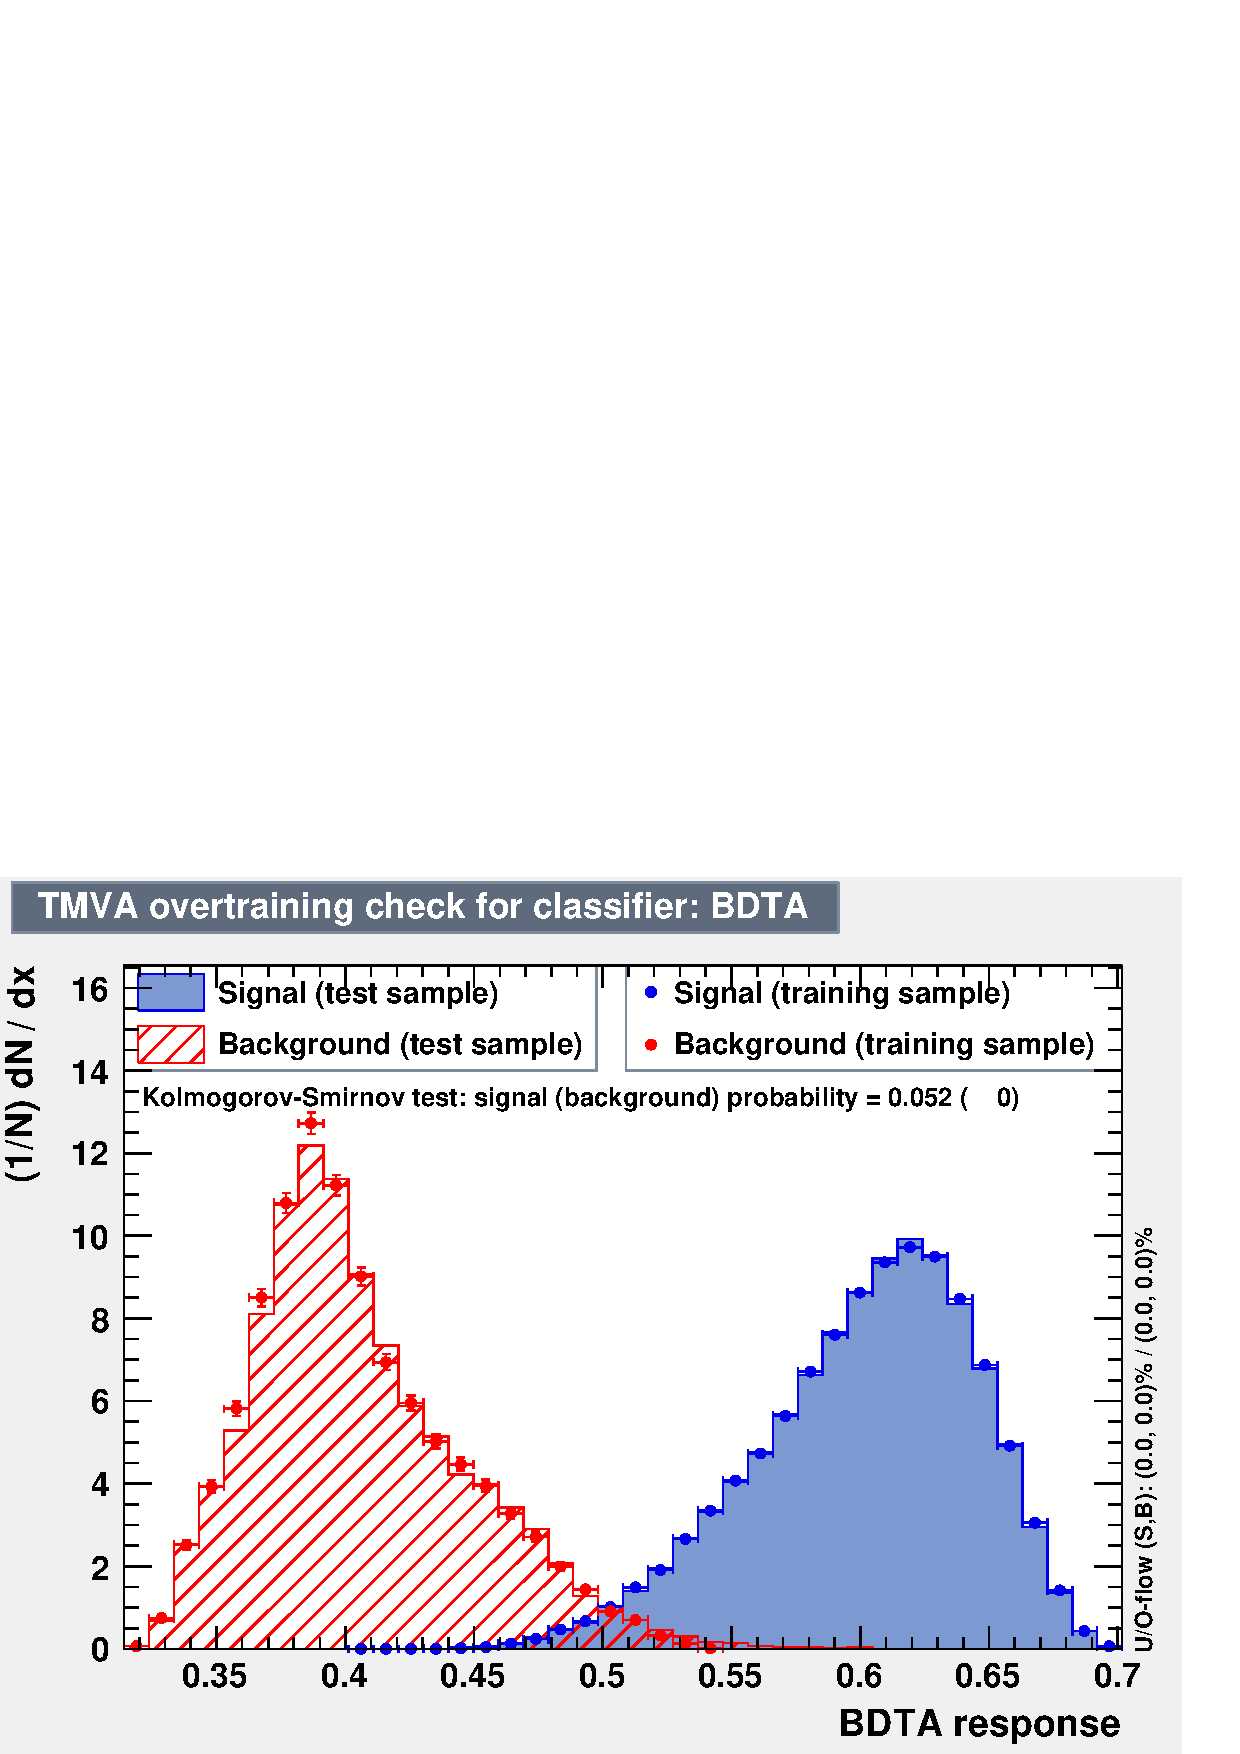
\includegraphics[width=0.8\textwidth]{figures/CosBDT/BDTPost.png}
  \caption[Cosmic Rejection BDT Output Distributions]{The cosmic rejection BDT output distributions for later data taking periods that encompass the majority of the data. The training sample is only $\numu$ CCs and the background sample is only cosmic trigger data events. Other beam events tend to have a similar distribution to the signal.}
  \label{fig:PIDCosBDT}
\end{figure}

\subsection{CVN, the All Purpose PID}
\label{sec:PIDCVN}

CVN, discussed in detail in reference \cite{ref:CVN}, does not attempt to identify a single event type; rather, it gives the most likely event type among all possibilities. CVN, or convolutional visual network, is the specific application of a CNN, or convolutional neural network, a deep learning technique that has had success in the field of computer vision and specifically in image processing and classification. CVN was developed as a classifier for \nova~as the events in each view are essentially images of physics processes.

One of the advantages of CNNs is that they do not require a known set of features as inputs; instead, the CNN itself finds and trains on the image features. CNNs use a stack of kernels within a convolutional layer to transform an image in a variety of ways, where each kernel can be thought of as finding a particular feature. For a layer $f$ that acts on an $n\times m$ set of pixels from an image $g$, the image is transformed via
\beq
(f \ast g)_{p,q,r} = \sum_{i=1}^n \sum_{j=1}^m \sum_{k=1}^c f_{i,j,k,r} g_{p+i,q+j,k},
\label{eq:CVNKernel}
\eeq

\n where $p$ and $q$ are the output pixel indices, $r$ is the output channel, $k$ is the input channel, and $c$ is the total number of channels. For a traditional image, channels refer to the RGB values of the pixel. In \nova, the pixels are the individual cells and the channels are the two views of the event. The energy deposited in a cell is encoded into an $8$-bit integer with $256$ possible values much like the intensities of a standard color are encoded. After the kernel is applied to the full image, the output is called a feature map, and a separate map is created and stored from each of the $r$ kernels in the convolutional layer. 

CNNs contain many layers that perform different functions. Convolutional layers nearest to the input image tend to output feature maps that exaggerate specific features while later layers become more holistic and topological. Other layers down-sample the image using a pooling technique that replaces an $n\times m$ subset of pixels with either the maximum pixel value (max pooling) or the average pixel value (average pooling). Finally, a process called local response normalization (LRN) is used that normalizes the result of a given pixel in a feature map relative that pixel in adjacent maps to avoid local minima.

The different layers are chained together into a particular architecture. CVN was built as a modified version of the GoogLeNet \cite{ref:GoogLeNet} architecture using the Caffe \cite{ref:Caffe} framework. One of the features of the GoogLeNet architecture used in several layers for CVN is the inception module, shown in figure \ref{fig:CVNInception}. This module performs several parallel feature extractions at different scales before concatenating the results into a single output layer. The full architecture of CVN is shown in figure \ref{fig:CVNArchitecture}. The XZ and YZ views are split and passed through two independent, equivalent branches. The output from these branches are only joined toward the end of the chain. The output of the final CVN inception module layer is passed into a traditional network for classification, where the event type outputs are normalized to $1$ to be interpreted as probabilities.
\begin{figure}[htb]
  \centering
  \includegraphics[width=0.8\textwidth]{figures/CVN/Inception.png}
  \caption[Inception Module Schematic]{Schematic of the Inception module.}
  \label{fig:CVNInception}
\end{figure}

\begin{figure}[p]
  \centering
  \includegraphics[width=0.55\textwidth]{figures/CVN/Architecture.png}
  \caption[CVN Architecture Schematic]{Schematic of the CVN architecture. The algorithm starts at the bottom and moves upward.}
  \label{fig:CVNArchitecture}
\end{figure}

CNNs are trained by using a set of images with known classifications and by optimizing a set of weights for each feature to minimize a loss function. This was done for CVN in two steps \cite{ref:TNCVN}, first training over a set of MC events, and second adding in cosmic data. The MC events were split into $13$ types, \{$\numu$ CC, $\nue$ CC, $\nutau$ CC\} $\times$ \{QE, RES, DIS, Other\} and NC. After the training weights for these event types stabilized, a sample of cosmic trigger data was added to train the PID with the full suite of event types. The cosmics were added in a separate step to prevent the PID from simply learning to reject data. Instead of using the entire detector view as the initial input, a smaller $100$ plane $\times$ $80$ cell view is constructed with the most upstream plane lining up with the first hit and the cells centered on the median hit for training, testing, and evaluation.

A true NC, $\nue$ CC, and $\numu$ CC event are each shown with a corresponding feature map collection in figure \ref{fig:CVNEvents}. The maps shown are from the output of the first inception module for the YZ view. Three particular features are highlighted for each of these events that appear to correspond to traditional features. The green feature map shows activity for the $\numu$ CC event as a long, track like feature. Unsurprisingly, this feature map shows little activity for the other two events. The blue map shows a more diffuse pattern for the $\nue$ CC event, but is almost entirely absent for the $\numu$ CC and NC events. This feature map thus appears to be picking out the characteristic shower development of electrons. Finally, the pink map shows moderate activity for all events, with a small peak of activity in the center of the left edge. This feature map seems to be sensitive to the hadronic activity near the event vertex. To reiterate, these feature maps are not the inputs into the final classification layer, but to another inception module layer. As the layers become deeper, the extracted features become more abstract. Distributions of the NC classifier are shown in section \ref{sec:SelNCSel} on NC event selection, section \ref{sec:ResultsND} on ND data/MC comparisons, and section \ref{sec:ResultsFD} on the final results.
\begin{figure}[p]
  \centering
  \begin{tabular}{c}
    \includegraphics[width=.95\textwidth]{figures/CVN/MapNumu.png} \\
    \includegraphics[width=.95\textwidth]{figures/CVN/MapNue.png} \\
    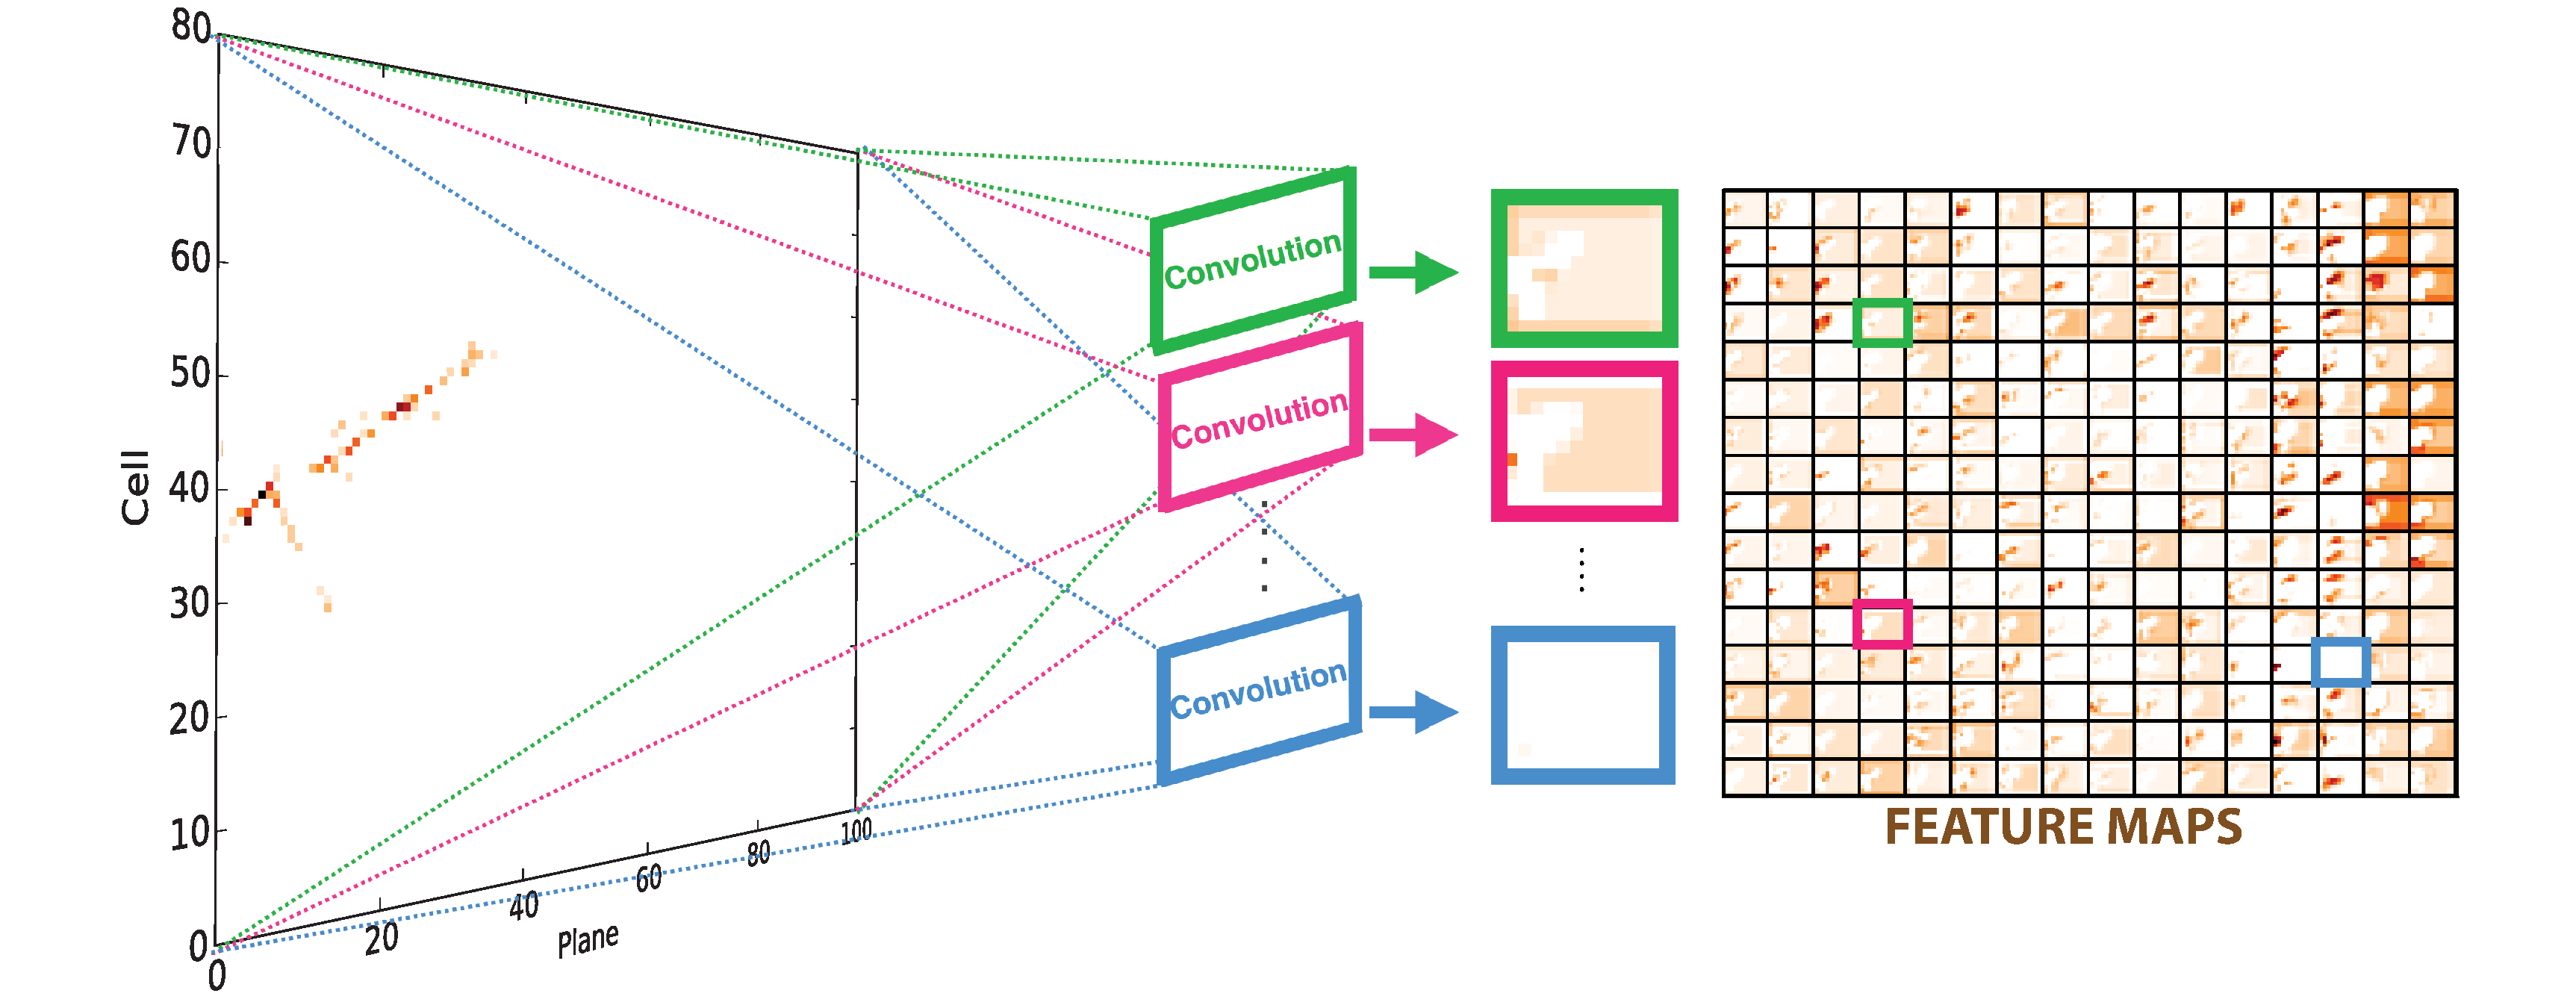
\includegraphics[width=.95\textwidth]{figures/CVN/MapNC.png} \\
  \end{tabular}
  \caption[Feature Maps from Representative Events]{Feature maps from representative events. Top: True $\numu$ CC. Middle: True $\nue$ CC. Bottom: True NC.}
  \label{fig:CVNEvents}
\end{figure}